\documentclass[tikz,border=6pt]{standalone}
\usepackage[T1]{fontenc}
\usepackage{helvet}
\renewcommand{\familydefault}{\sfdefault}
\usepackage{tikz}
\usepackage{pgfplots}
\pgfplotsset{compat=1.18}

\definecolor{ink}{HTML}{1F2937}
\definecolor{muted}{HTML}{6B7280}
\definecolor{head}{HTML}{1E3A5F}
\definecolor{bar}{HTML}{047857}

\begin{document}
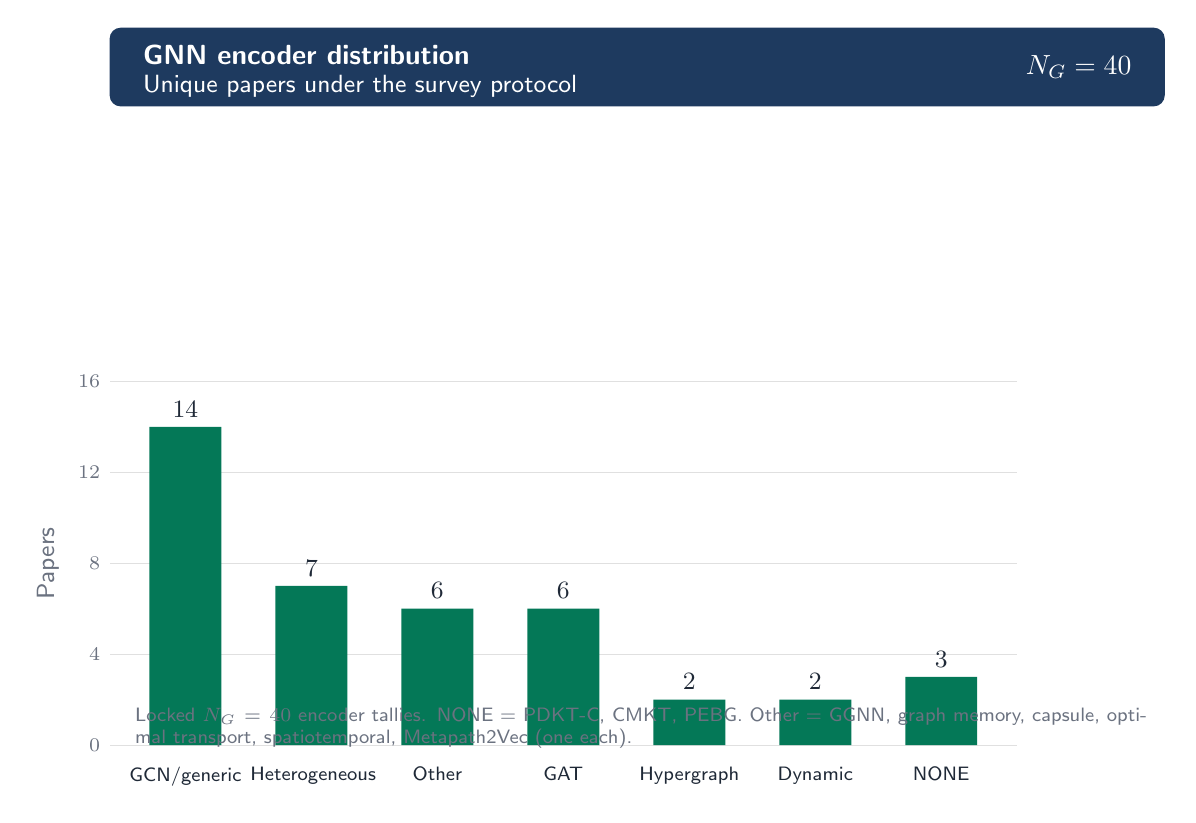
\begin{tikzpicture}
\fill[head, rounded corners=4pt] (0,8.15) rectangle (13.4,9.15);
\node[anchor=west, text=white, font=\sffamily\bfseries] at (0.30,8.80)
  {GNN~encoder~distribution};
\node[anchor=west, text=white!88, font=\sffamily\small] at (0.30,8.40)
  {Unique papers under the survey protocol};
\node[anchor=east, text=white, font=\sffamily\bfseries] at (13.10,8.65)
  {$N_G=40$};

\begin{axis}[
    at={(0.20,1.35)},
    ybar,
    bar width=26pt,
    ymin=0,
    ymax=16,
    width=13.1cm,
    height=6.2cm,
    axis line style={draw=none},
    tick style={draw=none},
    xtick=data,
    symbolic x coords={GCN/generic, Heterogeneous, Other, GAT, Hypergraph, Dynamic, NONE},
    x tick label style={font=\sffamily\scriptsize, text=ink, align=center, text width=1.55cm},
    ytick={0,4,8,12,16},
    y tick label style={font=\sffamily\scriptsize, text=muted},
    ylabel={Papers},
    ylabel style={font=\sffamily\small, text=muted},
    nodes near coords,
    every node near coord/.append style={font=\sffamily\bfseries\small, text=ink},
    ymajorgrids=true,
    xmajorgrids=false,
    major grid style={line width=0.3pt, draw=black!12},
]
\addplot[fill=bar, draw=none] coordinates {
    (GCN/generic,14)
    (Heterogeneous,7)
    (Other,6)
    (GAT,6)
    (Hypergraph,2)
    (Dynamic,2)
    (NONE,3)
};
\end{axis}

\node[anchor=west, text=muted, font=\sffamily\scriptsize, text width=13.0cm] at (0.20,0.25)
  {Locked $N_G=40$ encoder tallies. NONE = PDKT-C, CMKT, PEBG. Other = GGNN, graph memory, capsule, optimal transport, spatiotemporal, Metapath2Vec (one each).};
\end{tikzpicture}
\end{document}
